\documentclass[11pt,a4paper]{article}
\usepackage[utf8]{inputenc}
\usepackage[spanish,es-tabla]{babel}
\usepackage{geometry}
\geometry{top=2.5cm,bottom=2.5cm,left=2.5cm,right=2.5cm}
\usepackage{helvet}
\renewcommand{\familydefault}{\sfdefault}
\usepackage{graphicx}
\usepackage{booktabs}
\usepackage{tabularx}
\usepackage{microtype}
\usepackage{fancyhdr}
\usepackage{hyperref}

\hypersetup{
    colorlinks=false,
    pdfborder={0 0 0},
    pdfauthor={Yandris Rivera Torres},
    pdftitle={Actividad AA1-5: Endpoints Pedidos y Comparativa MVC, MVT, API-First}
}

\begin{document}

% =========================================================================
% CARÁTULA INSTITUCIONAL SOBRIA UPSE
% =========================================================================
\begin{titlepage}
    \centering
    \vspace*{-0.5cm}
    {\large \textbf{UNIVERSIDAD ESTATAL PENÍNSULA DE SANTA ELENA}}\\[0.25cm]
    {\textbf{FACULTAD DE SISTEMAS Y TELECOMUNICACIONES}}\\[0.2cm]
    {\textbf{CARRERA DE INGENIERÍA EN SOFTWARE}}\\[1.2cm]
    
    
\includegraphics[width=5.5cm]{docs/entregables/Actividad5/capturas/logo_upse.png}\\[1.2cm]
    
    {\small \textbf{ASIGNATURA:}}\\[0.15cm]
    {\large \textbf{FRAMEWORK PROGRAMACIÓN WEB}}\\[0.8cm]
    
    {\small \textbf{TEMA:}}\\[0.15cm]
    {\textbf{TRABAJO PRÁCTICO EXPERIMENTAL - ACTIVIDAD AA1-5}}\\[0.1cm]
    {\small Desarrollo de Endpoints en FastAPI, Validación con Pydantic y Cuadro Comparativo}\\[0.8cm]
    
    {\small \textbf{ELABORADO POR:}}\\[0.15cm]
    {\textbf{YANDRIS RIVERA TORRES}}\\[0.8cm]
    
    {\small \textbf{CURSO Y PARALELO:}}\\[0.15cm]
    {\textbf{SOFTWARE 7/1}}\\[0.8cm]
    
    {\small \textbf{DOCENTE:}}\\[0.15cm]
    {\textbf{ING. CARLOS EDUARDO MUÑOZ MENDOZA}}\\[1.2cm]
    
    \vfill
    {\small \textbf{LA LIBERTAD -- ECUADOR}}\\[0.1cm]
    {\footnotesize 2026 -- 2027}
\end{titlepage}

\newpage
\pagestyle{fancy}
\fancyhf{}
\renewcommand{\headrulewidth}{0.5pt}
\fancyhead[L]{\footnotesize Universidad Estatal Península de Santa Elena}
\fancyhead[R]{\footnotesize Framework Programación Web - Actividad AA1-5}
\fancyfoot[L]{\footnotesize Carrera de Ingeniería en Software}
\fancyfoot[R]{\footnotesize Página \thepage\ de 3}

% =========================================================================
% PÁGINA 2: CONTENIDO TÉCNICO FORMAL
% =========================================================================

\section*{Informe Técnico: Módulo de Pedidos y Aislamiento Multi-Tenant}
\noindent{\footnotesize \textbf{Rama de Trabajo:} \texttt{yandris-rivera/AA1-5} \quad \textbar \quad \textbf{Módulo:} \texttt{fastAPI\_SaaS} \quad \textbar \quad \textbf{Fecha:} Noviembre 2026}
\vspace{0.2cm}
\hrule
\vspace{0.4cm}

\subsection*{1. Implementación de Endpoints y Lógica de Negocio}
En \texttt{src/api-saas} se desarrolló el módulo de pedidos satisfaciendo los requerimientos solicitados:
\begin{enumerate}
    \item \textbf{\texttt{PUT /api/\{tenant\_id\}/pedidos/\{pedido\_id\}/estado}:} Modifica el estado del pedido a través de una máquina de estados finita (\texttt{pendiente} $\rightarrow$ \texttt{preparando} $\rightarrow$ \texttt{en\_camino} $\rightarrow$ \texttt{entregado} / \texttt{cancelado}). Ante una transición inválida (ej. cancelar un pedido entregado), responde con error \textbf{400 Bad Request}.
    \item \textbf{\texttt{DELETE /api/\{tenant\_id\}/pedidos/\{pedido\_id\}}:} Elimina el pedido garantizando aislamiento entre tiendas (retorna \textbf{204 No Content}). Si el pedido pertenece a otra tienda, responde \textbf{404 Not Found} para impedir la enumeración y filtración de recursos entre inquilinos.
\end{enumerate}

\subsection*{2. Reglas de Validación Declarativa con Pydantic v2}
En \texttt{app/modules/pedidos/schemas.py} se implementó la validación estricta de datos de entrada:
\begin{itemize}
    \item \texttt{cantidad: int = Field(..., gt=0)}: Rechaza cualquier cantidad menor o igual a cero con código \textbf{422 Unprocessable Entity}.
    \item \texttt{total: Decimal = Field(..., gt=0)}: Rechaza importes menores o iguales a cero con código \textbf{422}.
    \item \textbf{Capa de Persistencia:} La migración \texttt{0005\_pedidos.py} refuerza la integridad mediante \texttt{CHECK (cantidad > 0 AND total > 0)}.
    \item \textbf{Aislamiento:} Triple barrera mediante alcance del token (403), filtro de repositorio por \texttt{tenant\_id} (404) y Row-Level Security (RLS) en PostgreSQL con \texttt{SET LOCAL app.current\_tenant}.
\end{itemize}

\vspace{0.3cm}

\subsection*{3. Cuadro Comparativo de Enfoques Arquitectónicos}

\noindent
\begin{tabularx}{\textwidth}{p{3.2cm} X X X}
\toprule
\textbf{Criterio} & \textbf{MVC Clásico} & \textbf{MVT (Django)} & \textbf{API-First (FastAPI)} \\
\midrule
\textbf{Organización} & Controlador + Vista + Modelo & Modelo + Template + Vista & Recurso + Schema + Router \\
\addlinespace
\textbf{Entrada Usuario} & Formulario POST tradicional & Formulario renderizado servidor & Payload JSON sobre HTTP \\
\addlinespace
\textbf{Validación} & Manual en controlador o modelo & Formularios Django (\texttt{ModelForm}) & \textbf{Pydantic v2 en el borde} (\texttt{gt=0}) \\
\addlinespace
\textbf{Contrato API} & Implícito acoplado a la vista & Implícito acoplado a templates & \textbf{OpenAPI / Swagger explícito} \\
\addlinespace
\textbf{Formato Respuesta} & Páginas HTML completas & HTML procesado con motor DTL & JSON estándar desacoplado \\
\addlinespace
\textbf{Multi-tenancy} & Filtro manual por consulta & Filtro manual en manager & Inyección dependencias + RLS Postgres \\
\addlinespace
\textbf{Testabilidad} & Servidor HTTP completo & Requiere \texttt{django.test.Client} & \texttt{ASGITransport} in-process veloz \\
\addlinespace
\textbf{Acoplamiento} & Alto entre Vista y Controlador & Alto entre Template y Modelo & \textbf{Bajo}: Dominio y contratos libres \\
\addlinespace
\textbf{Caso de Uso} & Sitios monolíticos web & Portales con CMS y administración & \textbf{SaaS multi-cliente} (Web, Móvil, APIs) \\
\bottomrule
\end{tabularx}

\vspace{0.3cm}
\noindent\textbf{Análisis Técnico:} MVC y MVT fueron diseñados para la entrega de vistas server-side. En contraposición, API-First convierte al contrato OpenAPI en la base de la solución: la validación ocurre de manera inmediata en el borde antes de llegar a la base de datos, posibilitando que una sola API dé servicio a clientes web, móviles y externos.

\newpage

% =========================================================================
% PÁGINA 3: EVIDENCIAS EN /DOCS, PRUEBAS Y CONCLUSIÓN
% =========================================================================

\subsection*{4. Evidencias de Pruebas y Contrato en /docs}
La especificación interactiva OpenAPI generada automáticamente por FastAPI documenta las rutas implementadas y las restricciones numéricas de los esquemas:

\begin{figure}[h!]
    \centering
    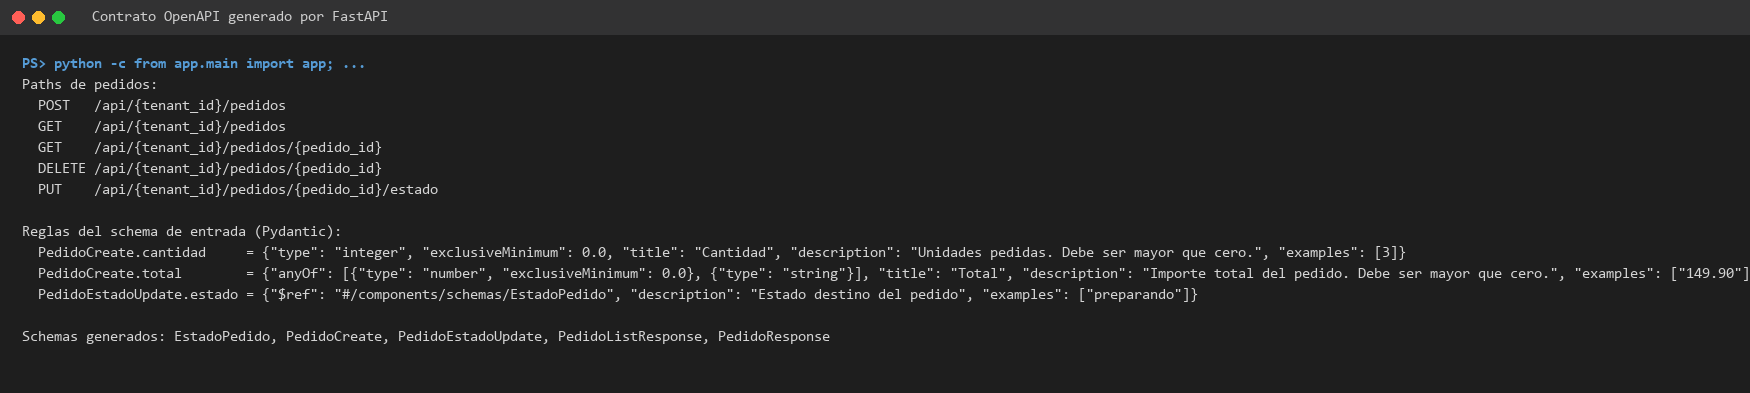
\includegraphics[width=0.95\textwidth]{docs/entregables/Actividad5/capturas/openapi_pedidos.png}
    \caption{Especificación interactiva OpenAPI (/docs) con las operaciones de Pedido.}
\end{figure}

\subsection*{5. Verificación Automatizada (Pytest)}
Resultados de la batería de pruebas unitarias y de integración:

\begin{figure}[h!]
    \centering
    \begin{minipage}{0.55\textwidth}
        \centering
        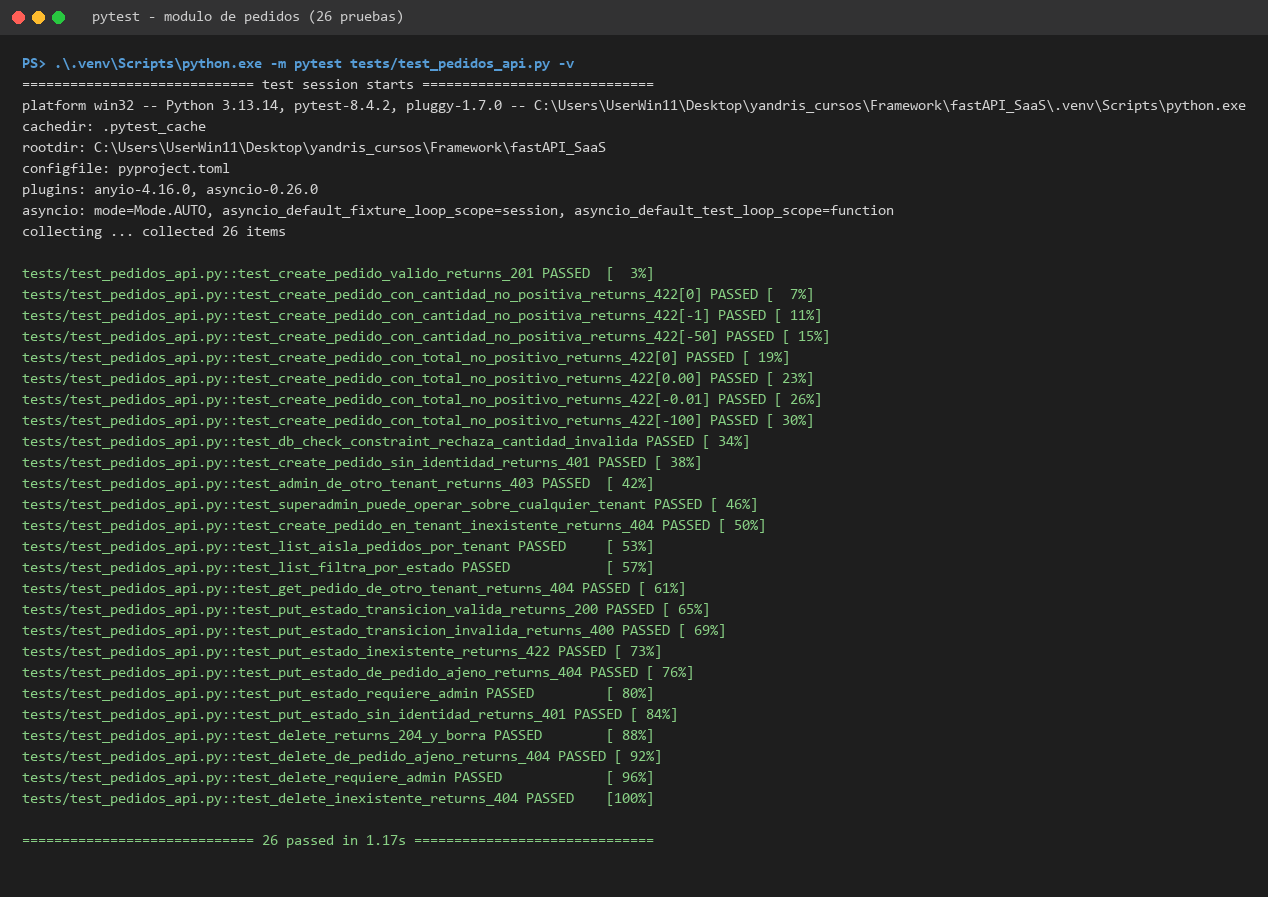
\includegraphics[width=\linewidth]{docs/entregables/Actividad5/capturas/pytest_pedidos.png}
        \caption{26 pruebas de pedidos (gt=0, RLS, 404/403).}
    \end{minipage}
    \hfill
    \begin{minipage}{0.42\textwidth}
        \centering
        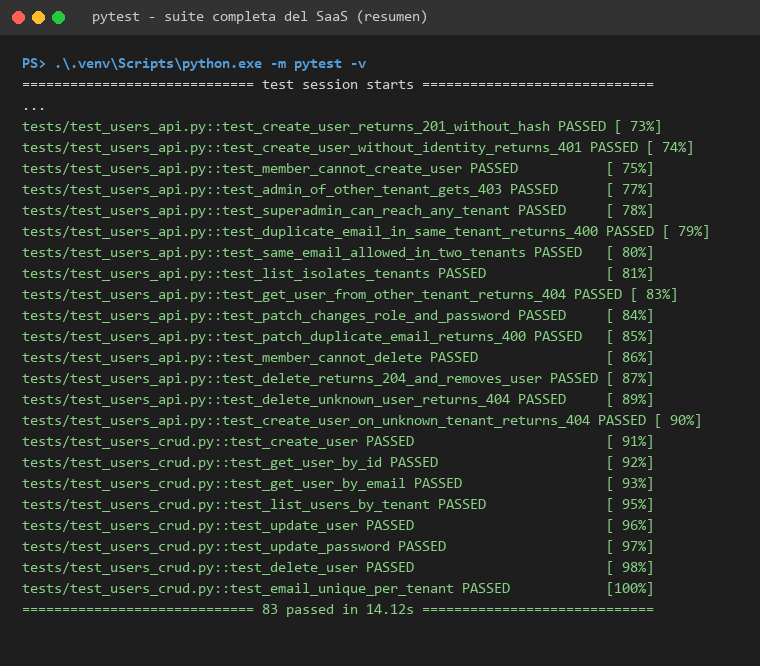
\includegraphics[width=\linewidth]{docs/entregables/Actividad5/capturas/pytest_suite_resumen.png}
        \caption{Suite completa SaaS: 83 tests en verde.}
    \end{minipage}
\end{figure}

\subsection*{6. Conclusiones}
\begin{itemize}
    \setlength{\itemsep}{2pt}
    \item \textbf{Endpoints Solicitados:} \texttt{PUT /estado} y \texttt{DELETE} implementados con máquina de estados finita y aislamiento absoluto por tienda.
    \item \textbf{Validación Perimetral:} Pydantic v2 intercepta peticiones con cantidad o total $\le 0$ con código \textbf{422 Unprocessable Entity}.
    \item \textbf{Aislamiento Multi-Tenant:} Triple garantía con verificación de tokens (403), repositorio filtrado (404) y Row-Level Security en PostgreSQL.
    \item \textbf{Calidad de Software:} 83 pruebas pasadas satisfactoriamente aseguran la ausencia de regresiones en la plataforma.
\end{itemize}

\vspace{0.4cm}
\hrule
\vspace{0.2cm}
\noindent{\footnotesize \textbf{Repositorio Oficial Git:} \url{https://github.com/yan2005dris-afk/Framework} \quad \textbar \quad \textbf{Rama:} \texttt{yandris-rivera/AA1-5}}

\end{document}
